\documentclass[letterpaper]{article}
\usepackage[spanish]{babel}
\usepackage{fixltx2e}
\usepackage{graphicx}
\usepackage[utf8]{inputenc}
\usepackage{hyperref}
\usepackage{mathtools}
\usepackage{numprint}
\usepackage{tabu}

\npthousandsep{\thinspace}
\npthousandthpartsep{}
\npdecimalsign{,}

\begin{document}

\title{Evaluación del informe\\"Generación de códigos únicos para unidades geográficas"}
\author{Sylvain Lesage\\
  \texttt{slesage@adsib.gob.bo}}
\date{\today}
\maketitle
 
\begin{abstract}
Abstract...
\end{abstract}

\section{Antecedentes}

El Instituto Nacional de Estadísticas (INE) esta trabajando en una 
nueva codificación de los lugares, en particular localidades, 
comunidades y manzanos. El actual código tiene el problema de depender 
de la situación administrativa del lugar, por ejemplo el código 
actual contiene el código del departamento y del municipio. Es un 
problema en varias localidades o comunidades para las cuales la 
situación administrativa, en particular la dependencia a tal o tal 
municipio, no esta consensuada. Por esta razón, el INE decidió 
generar un nuevo código, basado únicamente en la ubicación 
geográfica del lugar, es decir la latitud y la longitud de un punto, 
que puede ser el centroide del territorio.

En el marco de las relaciones inter-institucionales entre el INE y la 
ADSIB, el equipo técnico del INE nos propuso revisar su propuesta de 
nuevo código. En este informe, describimos nuestra evaluación, y 
proponemos alternativas.

\section{Problemática}
\label{sec:problematica}

El nuevo código INE busca resolver el problema siguiente:

\begin{quote}
codificar la ubicación de un punto geográfico, de manera única, en 
un número mínimo de caracteres.
\end{quote}

Algunas características deseables del código son:
\begin{itemize}
	\item código compacto: utilizar el número mínimo de caracteres, 
	que sean números o letras, para codificar la ubicación.
	\item precisión alta: reducir la superficie de las zonas de mismo 
	código a lo mínimo.\footnote{Hay que notar que el código no puede 
	ser único. En efecto, la codificación consiste a dividir el 
	territorio nacional, o sea una superficie continua, en un número 
	finito de códigos, cada código correspondiendo a una zona 
	definida. Más que buscar un hipotético código único, se trata de 
	definir el \emph{nivel de precisión} del código: por ejemplo, 
	¿que es la superficie de las zonas de mismo código? Un nivel de 
	precisión alto corresponde a una zona pequeña, por ejemplo: \(
	10\,\mathrm{m}\) por \(10\,\mathrm{m}\).}
	\item forma adecuada de las zonas de mismo código: puede ser un 
	cuadrado en el sistema latitud/longitud, un rectángulo, u otras 
	formas. Lo más lógico es que la forma sea la más compacta 
	posible alrededor del centroide.
	\item nivel de precisión incremental: idealmente, 
	los primeros caracteres del código expresan la ubicación a un 
	nivel de precisión bajo, y cada nuevo carácter aumenta el nivel de 
	precisión.
	\item simplicidad del cálculo: el cálculo debe ser lo más 
	simple, a partir de los datos más comunes para la ubicación de 
	puntos, es decir latitud y longitud en el sistema WGS84\footnote
	{WGS84 es el estándar utilizado en el sistema GPS, ver \url
	{https://en.wikipedia.org/wiki/World_Geodetic_System.}}
	\item simplicidad de los cálculos conexos: en particular, el 
	código debe ser diseñado de manera a facilitar el cálculo de 
	proximidad entre dos localidades.
	\item respaldo científico: la publicación de la definición del 
	código en la literatura científica es un buen indicador de su 
	calidad.
	\item herramientas disponibles: una abundante lista de 
	herramientas compatibles con el código es una ventaja para su uso 
	masivo y para la conversión del actual código al nuevo código.
\end{itemize}

\section{Características de la propuesta de nuevo código INE}

La propuesta de nuevo código proveída por el INE se encuentra en 
anexo. Lo anotaremos \(z\) en las ecuaciones.

\subsection{Definición del código \(z\)}

Dados \(x\) y \(y\) las coordenadas de un punto en la proyección 
cónica conforme de Lambert (PCCL)\cite[p.~33]{sunit07}, el código \(z\) 
esta definido\footnote{El documento base omite la adición de \(\pi\) 
en el cálculo de \(\theta\). Lo añadimos para que nuestros cálculos 
correspondan a los resultados proveídos por el equipo técnico del 
INE.} por:

\[z = \lfloor r \exp{\theta} \rfloor\]

con

\[
\left\{
\begin{array}{l l}
r = \sqrt{x^2+y^2} \\
\theta = \arctan{\frac{y}{x}} + \pi
\end{array} \right.
\]

\subsection{Número de códigos \(z\) en Bolivia}

A partir del archivo de los límites de Bolivia\cite
{datos:limites_bolivia}, podemos calcular los valores límites de las 
coordenadas \(x\) y \(y\) de todos los puntos del territorio en la 
PCCL. La coordenada \(x\) se 
encuentra en el intervalo \([\numprint{391248}\,\mathrm{m}, 
\numprint{1689926}\,\mathrm{m}]\) y la coordenada \(y\) en el 
intervalo \([\numprint{119437}\,\mathrm{m}, 
\numprint{1583581}\,\mathrm{m}]\).

Podemos deducir el valor límite de las variables polares \(r\) y \(
\theta\). Tomar en cuenta que son valores límites, correspondiendo a 
las esquinas del \emph{bounding box} (cuadrado delimitado por \(
x_{min}\), \(x_{max}\), \(y_{min}\) y \(y_{max}\)) de Bolivia: no 
necesariamente existe un punto con estos valores de \(r\) y \(\theta
\). El radio \(r\) se encuentra en el intervalo \(
[\numprint{614506}\,\mathrm{m}, \numprint{1814299}\,\mathrm{m}]\) y 
el ángulo \(\theta\) en el intervalo \(
[\numprint{3.27}\,\mathrm{rad}, \numprint{4.44}\,\mathrm{rad}]\).

Según la formula de cálculo del código \(z\), esté crece con \(r\) y 
\(\theta\), por lo cual podemos calcular los valores límites del 
código \(z\) (con la misma advertencia: no necesariamente existe un 
punto en Bolivia que tenga estos valores extremos del código). Las 
estimaciones mínima y máxima del código \(z\) son respectivamente \(
\numprint{17493127}\) y \(\numprint{126692164}\). Por ende, podemos 
concluir que existe, en el territorio Boliviano, como estimación 
superior, \(\numprint{109199037}\) códigos diferentes.

El cuadro \ref{tab:variables} presenta un resumen de todos los valores.

\begin{table}
	\centering
	\begin{tabu} to \linewidth {|l|l|}
		\hline
		Variable & Valores \\
		\hline
		\(x\) & entre \(\numprint{391248}\,\mathrm{m}\) y \(\numprint{1689926}\,\mathrm{m}\) \\
		\(y\) & entre \(\numprint{119437}\,\mathrm{m}\) y \(\numprint{1583581}\,\mathrm{m}\) \\
		\hline
		\(r\) & entre \(\numprint{614506}\,\mathrm{m}\) y \(\numprint{1814299}\,\mathrm{m}\) \\
		\(\theta\) & entre \(3.27\,\mathrm{rad}\) y \(4.44\,\mathrm{rad}\) \\
		\hline
		código \(z\) & entre \(\numprint{17493127}\) y \(\numprint{126692164}\) \\
		número de códigos \(z\) & menos de \(\numprint{109199037}\) códigos diferentes \\
		\hline
	\end{tabu}
	\caption{Número de códigos \(z\) diferentes en Bolivia}
	\label{tab:variables}
\end{table}

\subsection{Precisión espacial del código \(z\)}

Tomando en cuenta que la superficie del territorio de Bolivia 
\footnote{según http://es.wikipedia.org/wiki/Bolivia} es 
aproximadamente de \(\numprint{1098581}\,\mathrm{km^{2}}\), podemos 
calcular que la superficie promedio del territorio correspondiendo a 
cada valor del código \(z\) es de \(\numprint{10060}\,\mathrm{m^{2}}
\), lo cual equivale un cuadrado de \(100\,\mathrm{m}\) de lado. 
Significa que para valor del código \(z\), existe una hectárea del 
territorio nacional donde todos los puntos comparten el mismo valor 
de \(z\), o sea donde el código \(z\) no permite discriminar entre 
los puntos incluidos. Podemos expresar este valor como el nivel de 
precisión del código \(z\). Los datos están presentados en el cuadro 
\ref{tab:precision}.

\begin{table}
	\centering
	\begin{tabu} to \linewidth {|l|l|}
		\hline
		Variable & Valores \\
		\hline
		superficie de Bolivia & \(\numprint{1098581}\,\mathrm{km^{2}}\) \\
		precisión del código  \(z\) & \(\numprint{10060}\,\mathrm{m^{2}}\), o sea una hectárea, como promedio\\
		\hline
	\end{tabu}
	\caption{Precisión espacial del código \(z\)}
	\label{tab:precision}
\end{table}

\subsection{Forma espacial de las zonas equi-código \(z\)}

Podemos también calcular la forma de las áreas \emph{equi-código} \(z\). 
Los límites de estas áreas son definidos, para un valor específico 
de \(z\), y para los ángulos \(\theta\) correspondiendo a Bolivia, 
por los valores siguientes:

\[
\left\{
\begin{array}{l l}
r_{min} = z \exp{-\theta} \\
r_{max} = (z+1) \exp{-\theta}
\end{array} \right.
\]

Calculamos la geometría de las nueve áreas correspondiendo al código 
de cada capital departamental de Bolivia. La figura \ref
{fig:areas_por_capital} representa estas áreas. Aparece claramente 
que les áreas \emph{equi-código} forman \emph{franjas} muy estrechas 
que cruzan toda Bolivia. Por ejemplo, el área que contiene el punto 
central de La Paz mide \(\numprint{1224}\,\mathrm{km}\) de largo y 
solamente \(\numprint{2.24}\,\mathrm{cm}\) de ancho en promedio (con 
un ancho mínimo de \(\numprint{1.18}\,\mathrm{cm}\) y un ancho 
máximo de \(\numprint{3.80}\,\mathrm{cm}\)). Su superficie es de \(
\numprint{19292}\,\mathrm{m^{2}}\), lo que equivale a un cuadrado de 
\(\numprint{138}\,\mathrm{m}\) de lado.

\begin{figure}[p]
    \centering
    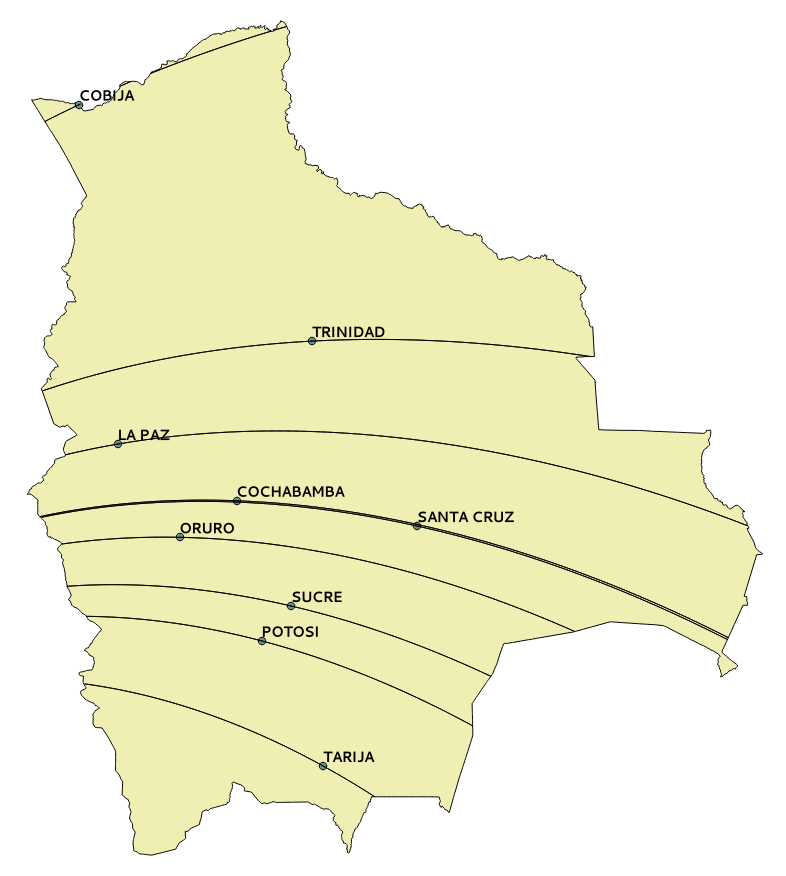
\includegraphics[width=0.8\textwidth]{resultados/area_equi_codigo_9_capitales.png}
    \caption{Área \emph{equi-código} para cada capital departamental de Bolivia. Nota: las áreas parecen líneas porque son extremadamente estrechas (\(\numprint{2.24}\,\mathrm{cm}\) en promedio)}
    \label{fig:areas_por_capital}
\end{figure}

El detalle de estas medidas para las nueve capitales de Bolivia se 
encuentra en el cuadro \ref{tab:capitales}. La figura \ref
{fig:areas_por_capital} y su acercamiento en la ciudad de Santa Cruz 
(figura \ref{fig:areas_por_capital_santacruz_cochabamba}) muestran 
que por casualidad, las áreas \emph{equi-código} \(z\) de Santa Cruz y 
Cochambamba casi se superponen, lo que significa que posiblemente 
varios manzanos de Santa Cruz y de Cochabamba compartan el mismo 
código.

\begin{table}
	\centering
	\begin{tabu} to \linewidth {|l|l|l|l|l|}
		\hline
		Capital & Superficie & Eq. lado de cuadrado & Largo & Ancho (promedio) \\
		\hline
		Cobija & \(\numprint{3377}\,\mathrm{m^{2}}\) & \(\numprint{58}\,\mathrm{m}\) & \(\numprint{352}\,\mathrm{km}\) & \(\numprint{2.24}\,\mathrm{cm}\) \\
		Trinidad & \(\numprint{12957}\,\mathrm{m^{2}}\) & \(\numprint{113}\,\mathrm{m}\) & \(\numprint{983}\,\mathrm{km}\) & \(\numprint{2.24}\,\mathrm{cm}\) \\
		La Paz & \(\numprint{19292}\,\mathrm{m^{2}}\) & \(\numprint{113}\,\mathrm{m}\) & \(\numprint{1224}\,\mathrm{km}\) & \(\numprint{2.24}\,\mathrm{cm}\) \\
		Cochabamba & \(\numprint{21072}\,\mathrm{m^{2}}\) & \(\numprint{145}\,\mathrm{m}\) & \(\numprint{1244}\,\mathrm{km}\) & \(\numprint{2.24}\,\mathrm{cm}\) \\
		Oruro & \(\numprint{15302}\,\mathrm{m^{2}}\) & \(\numprint{145}\,\mathrm{m}\) & \(\numprint{919}\,\mathrm{km}\) & \(\numprint{2.24}\,\mathrm{cm}\) \\
		Sucre & \(\numprint{13106}\,\mathrm{m^{2}}\) & \(\numprint{114}\,\mathrm{m}\) & \(\numprint{760}\,\mathrm{km}\) & \(\numprint{2.24}\,\mathrm{cm}\) \\
		Potosí & \(\numprint{12907}\,\mathrm{m^{2}}\) & \(\numprint{113}\,\mathrm{m}\) & \(\numprint{701}\,\mathrm{km}\) & \(\numprint{2.24}\,\mathrm{cm}\) \\
		Tarija & \(\numprint{10864}\,\mathrm{m^{2}}\) & \(\numprint{104}\,\mathrm{m}\) & \(\numprint{540}\,\mathrm{km}\) & \(\numprint{2.24}\,\mathrm{cm}\) \\
		Santa Cruz & \(\numprint{21064}\,\mathrm{m^{2}}\) & \(\numprint{145}\,\mathrm{m}\) & \(\numprint{1241}\,\mathrm{km}\) & \(\numprint{2.24}\,\mathrm{cm}\) \\
		\hline
	\end{tabu}
	\caption{Área \emph{equi-código} para cada capital departamental de Bolivia}
	\label{tab:capitales}
\end{table}

\begin{figure}[p]
    \centering
    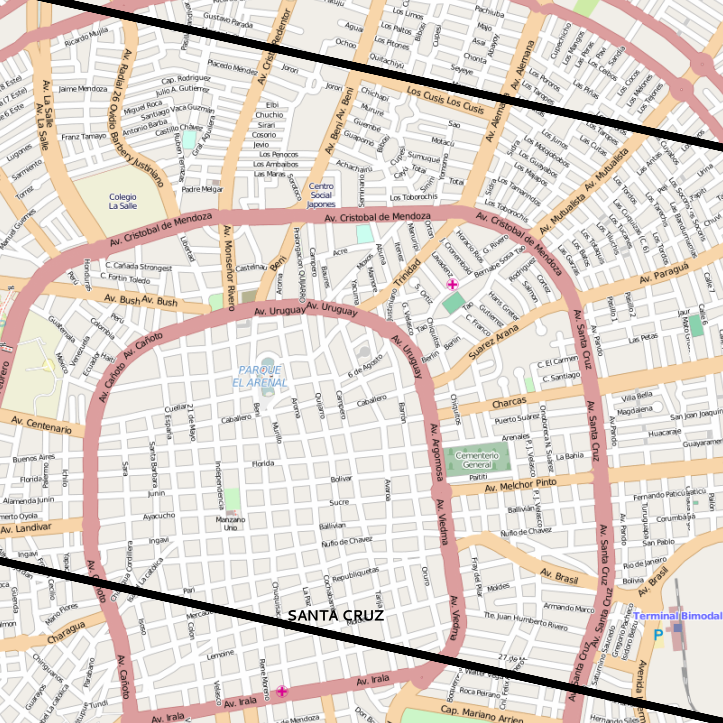
\includegraphics[width=0.8\textwidth]{resultados/area_equi_codigo_santacruz_cochabamba.png}
    \caption{Acercamiento sobre la ciudad de Santa Cruz para las áreas \emph{equi-código} para Santa Cruz y Cochabamba. Toda una franja de la ciudad de Santa Cruz (banda negra arriba) comparte el mismo código que la ciudad de Cochambamba}
    \label{fig:areas_por_capital_santacruz_cochabamba}
\end{figure}

\subsection{Otras características del código \(z\)}
\label{sec:otras_ine}

En la sección \ref{sec:problematica} definimos varios criterios de 
evaluación de una propuesta de código. En las secciones anteriores, 
detallamos los criterios de precisión y de forma de las zonas de mismo 
código. Evaluamos en esta sección los otros criterios para el código 
\(z\).

El código \(z\) esta compuesto únicamente de cifras, entre ocho y 
nueve cifras. En la propuesta del INE, este número de cifras no es configurable según el nivel 
de precisión deseado, es fijo y depende de la formula de definición 
del código \(z\). Sin embargo, podemos imaginar cambiar la definición 
para que sea configurable según un parámetro entero \(n\) que 
aumentará el nivel de precisión, y con él el tamaño del código:

\[z = \lfloor 10^{n} r \exp{\theta} \rfloor\]

A nivel de simplicidad del cálculo, la definición del código \(z\) 
obliga a calcular las coordenadas del punto en la PCCL.

La proximidad de dos códigos \(z\) permite establecer una proximidad 
aproximativa en el eje norte-sur (ver la figura \ref
{fig:areas_por_capital}) pero no da indicios sobre la proximidad en 
el eje oeste-este. En un ejemplo extremo, dos puntos ubicados 
respectivamente sobre la frontera con Perú y sobre la frontera con 
Brazil pueden tener el mismo código \(z\).

Finalmente, por su recién invención, el código \(z\) no ha sido 
publicado en la literatura científica y no existen herramientas para 
manejarlo.

El cuadro \ref{tab:carac_ine} presenta las características del código 
\(z\) de manera concisa.

\begin{table}
	\centering
	\begin{tabu} to \linewidth {|p{3cm}|p{8cm}|}
		\hline
		Criterio & Código \(z\) \\
		\hline
		código para la Paz & 61220260 \\
		\hline
		tamaño del código & 8 o 9 cifras (10 
		posibilidades por carácter) \\
		\hline
		duplicados (entre 80000 puntos) & ... \\
		\hline
		superficie equi-código con 9 caracteres (La Paz) & 
		\(\numprint{19292}\,\mathrm{m^{2}}\), 
		equivalente a un cuadrado de \(\numprint{113}\,\mathrm{m}\) de lado \\
		\hline
		forma equi-código (La Paz) & franja: 
		\(\numprint{1224}\,\mathrm{km}\) por 
		\(\numprint{2.24}\,\mathrm{cm}\) \\
		\hline
		configurar precisión & no esta 
		previsto, pero se podría implementar (ver \ref{sec:otras_ine}) \\
		\hline
		cálculo del código & necesita reproyectar de WGS84 en Lambert \\
		\hline
		cálculo de proximidad & fácil en un eje norte-sur, pero 
		imposible en un eje oeste-este \\
		\hline
		respaldo científico & ninguno\\
		\hline
		herramientas disponibles & ninguna \\
		\hline
	\end{tabu}
	\caption{Características del código \(z\)}
	\label{tab:carac_ine}
\end{table}

\section{Códigos alternativos}

La problemática expuesta en la sección \ref{sec:problematica} no es 
nueva y ha sido estudiada desde varias décadas, resultando en varias 
definiciones de códigos, utilizados en varios ámbitos. En las 
siguientes subsecciones presentamos algunos de los códigos más 
utilizados.

\begin{table}
	\centering
	\begin{tabu} to \linewidth {|p{3cm}|p{8cm}|}
		\hline
		Criterio & Código GeoHash\footnote{ver \url{http://en.wikipedia.org/wiki/Geohash}} \\
		\hline
		código para la Paz & 6mpd1mz3n \\
		\hline
		tamaño del código & variable - letras y cifras (36 
		posibilidades por carácter) \\
		\hline
		duplicados (entre 80000 puntos) & ... \\
		\hline
		superficie equi-código con 9 caracteres (La Paz) & 
		\(\numprint{21}\,\mathrm{m^{2}}\), 
		equivalente a un cuadrado de \(\numprint{4.6}\,\mathrm{m}\) de lado \\
		\hline
		forma equi-código (La Paz) & rectángulo: 
		\(\numprint{4.7}\,\mathrm{m}\) (norte-sur) por 
		\(\numprint{4.5}\,\mathrm{m}\) (oeste-este) \\
		\hline
		configurar precisión & sí, cada 
		carácter aumenta el nivel de precisión\footnote{ver 
		\url{http://en.wikipedia.org/wiki/Geohash\#Worked_example}} \\
		\hline
		cálculo del código & codificación de latitud y longitud en 
		base32 \\
		cálculo de proximidad & no es lo más adecuado\footnote{ver 
		\url{http://en.wikipedia.org/wiki/Geohash\#Limitations}} \\
		\hline
		respaldo científico & no encontré \\
		\hline
		herramientas disponibles & librerías para 15 lenguajes\footnote{ver 
		\url{http://en.wikipedia.org/wiki/Geohash\#External_links}} \\
		\hline
	\end{tabu}
	\caption{Características del código GeoHash}
	\label{tab:carac_geohash}
\end{table}

\begin{table}
	\centering
	\begin{tabu} to \linewidth {|p{3cm}|p{8cm}|}
		\hline
		Criterio & Código MGRS (Military grid reference system)\footnote{ver 
		\url{http://en.wikipedia.org/wiki/Military_grid_reference_system}} \\
		\hline
		código para la Paz & 19KEB9276 \\
		\hline
		tamaño del código & variable - 5 letras y cifras, luego cifras 
		por par \\
		\hline
		duplicados (entre 80000 puntos) & ... \\
		\hline
		superficie equi-código con 9 caracteres (La Paz) & 
		\(\numprint{1000000}\,\mathrm{m^{2}}\), 
		equivalente a un cuadrado de \(\numprint{1000}\,\mathrm{m}\) de lado \\
		\hline
		forma equi-código (La Paz) & rectángulo: 
		\(\numprint{1000}\,\mathrm{m}\) (norte-sur) por 
		\(\numprint{1000}\,\mathrm{m}\) (oeste-este) \\
		\hline
		configurar precisión & sí, cada dos 
		cifras dividen la superficie por 100 (o el lado del cuadrado 
		por 10)\footnote{ver 
		\url{http://en.wikipedia.org/wiki/Military_grid_reference_system}} \\
		\hline
		cálculo del código & conversión en UTM \\
		\hline
		cálculo de proximidad & ? \\
		\hline
		respaldo científico & DMA Technical Manual 8358.1, Chapter 3. Datums, Ellipsoids, Grids, and Grid Reference Systems \\
		\hline
		herramientas disponibles & librerías GeographicLib y 
		GeoConvert/mgrs en 9 lenguajes\footnote{ver 
		\url{https://pypi.python.org/pypi/mgrs} para python} \\
		\hline
	\end{tabu}
	\caption{Características del código MGRS}
	\label{tab:carac_mgrs}
\end{table}

\begin{table}
	\centering
	\begin{tabu} to \linewidth {|p{3cm}|p{8cm}|}
		\hline
		Criterio & Código MLocS (Maidenhead Locator System)\footnote{ver 
		\url{http://en.wikipedia.org/wiki/Maidenhead_Locator_System}} \\
		\hline
		código para la Paz & FH53WM32 \\
		\hline
		tamaño del código & variable, con letras y cifras \\
		\hline
		duplicados (entre 80000 puntos) & ... \\
		\hline
		superficie equi-código con 8 caracteres (La Paz) & 
		\(\numprint{1628640}\,\mathrm{m^{2}}\), 
		equivalente a un cuadrado de \(\numprint{1276}\,\mathrm{m}\) de lado \\
		\hline
		forma equi-código (La Paz) & rectángulo: 
		\(\numprint{1837}\,\mathrm{m}\) (norte-sur) por 
		\(\numprint{886}\,\mathrm{m}\) (oeste-este) \\
		\hline
		configurar precisión & sí, cada dos 
		cifras aumentan la precisión (un vez dividiendo por 10, la 
		otra por 24) \\
		\hline
		cálculo del código & codificación de las divisiones en grados, 
		minutos, etc. en WGS84 \\
		\hline
		cálculo de proximidad & ? \\
		\hline
		respaldo científico & R. J. Eckersley, G4FTJ (1985). Amateur Radio Operating Manual (third edition). Potters bar, UK: Radio Society of Great Britain. pp. 64–66. ISBN 0-900612-69-X. \\
		\hline
		herramientas disponibles & librerías en python (mlocs), perl, 
		y esta implementado en varios dispositivos GPS \\
		\hline
	\end{tabu}
	\caption{Características del código MLocS}
	\label{tab:carac_mlocs}
\end{table}

\begin{figure}[p]
    \centering
    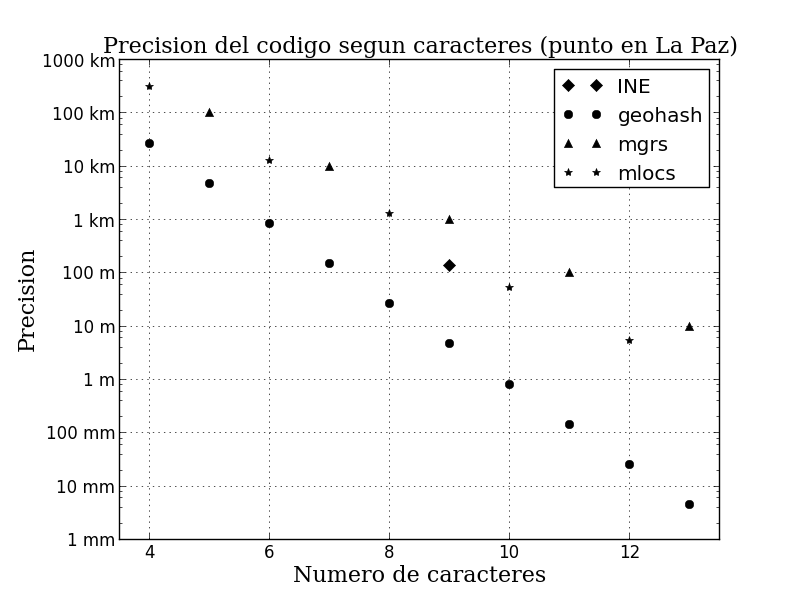
\includegraphics[width=0.8\textwidth]{resultados/precision_codigos.png}
    \caption{Precisión de los cuatro códigos (INE, Geohash, MGRS, 
    MLOCS) para el centro de La Paz, según el número de caracteres 
    en el código.}
    \label{fig:precision_codigos}
\end{figure}

\section{Conclusión y recomendaciones}



\begin{thebibliography}{99}

\bibitem{sunit07}
  Sistema Unico de Información de la Tierra,
  \emph{Normas técnicas para la administración de la información georeferenciada a nivel nacional}.
  Resolución Ministerial Nº~338 del MDRAyMA,
  2007.

\bibitem{datos:limites_bolivia}
  Límite Nacional de Bolivia,
  Formato Shapefile,
  GADM,
  \url{http://www.gadm.org},
  \url{http://biogeo.ucdavis.edu/data/gadm2/shp/BOL_adm.zip}

\end{thebibliography}

\end{document}
